%!TEX program = <xelatex>
\documentclass{book}
\usepackage{mystyle}
\begin{document}

\chapter{ Simulations and Results }\label{simulationsAndResults}

Recall that Liang-Wang example of a multimodial function:

\begin{equation}\label{againLiang}
f(x) = 
\sum_{i=1}^{20} \frac{\omega_i}{ \sigma_i \sqrt{2 \pi} } \exp \Big( -\frac{(x - \mu_i)^\tran (x - \mu_i)}{2 \sigma_i^2} \Big),	
\end{equation}
where $\sigma_1 = \dots = \sigma_{20} = 0.1$, $\omega_1 = \dots = \omega_{20} = 0.05 $ and the means $\mu_i$ are enlisted in Chapter \todo{Link with motivation}.

Since we are dealing with stochastic simulations, do focus on the first two empirical moments analysis of different statistics in order to get some understanding of which \textsc{Swap Strategies} is better. 
Because of theoretical reasons mentioned in the Chapter \todo{Theory}, one might be tempted to compare different \textsc{Swap Strategies} by considering the behaviour of their Колмогоров-Смирнов distance with the true underlying distribution, given by Eq. \ref{againLiang}. To this end the implemented KS statistics calculator was used, see \todo{Subsection on Колмогоров-Смирнов distance}. The overall results are gathered in Figure \ref{KSdistancePlot}. 
	
Unfortunately, the time-cost of the simulations that do calculate the KS statistics is quite long and so we did not manage to collect information on the same number of simulations. This might be a slight source of bias, especially when looking at statisctics such as the standard deviation. Even so one


\begin{figure}[ht]
	\centering 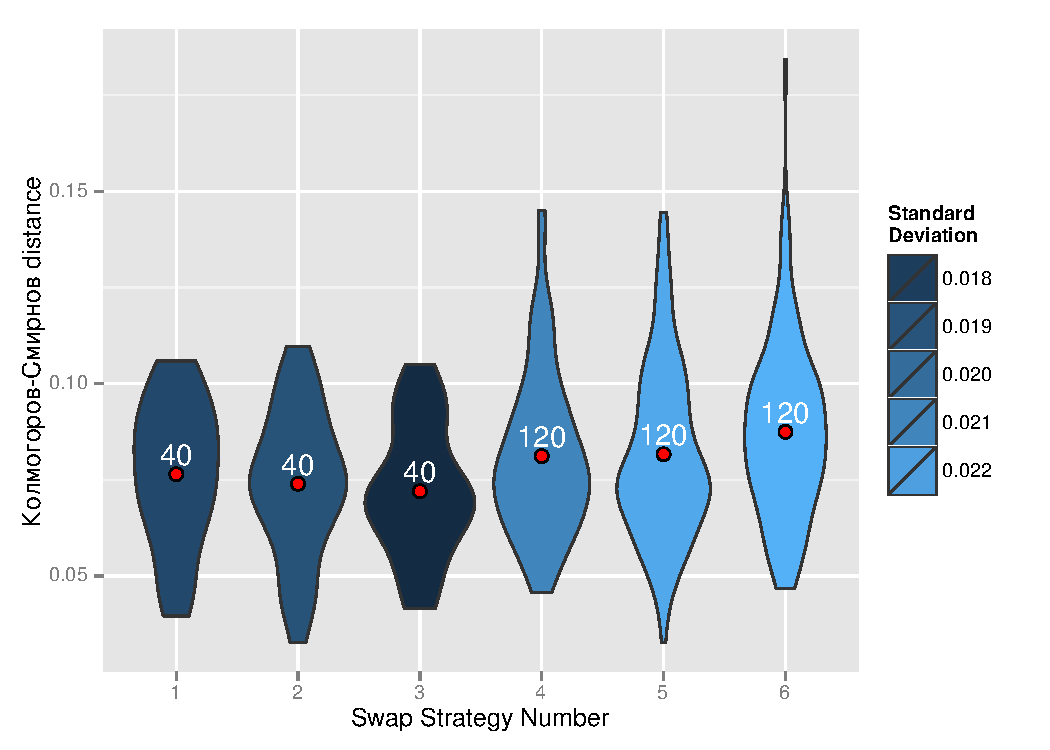
\includegraphics[width=\textwidth,keepaspectratio=TRUE]{./img/KSobs.pdf}
	\caption{Results of the KS statistiscs simulations. The number of iterations a particular strategy was tested is annotated with the white numbers just above the red dots. The violin plots are simply smoothened empirical distributions. Red dots are their empirical means. The colour of the violin plots corresponds to the standard deviation, which is more instructive to study when considering subgroups with the same number of simulations.}\label{KSdistancePlot}
\end{figure}


\section{Comparing ourselves with Baragatti}

\begin{figure}[ht]
	\centering 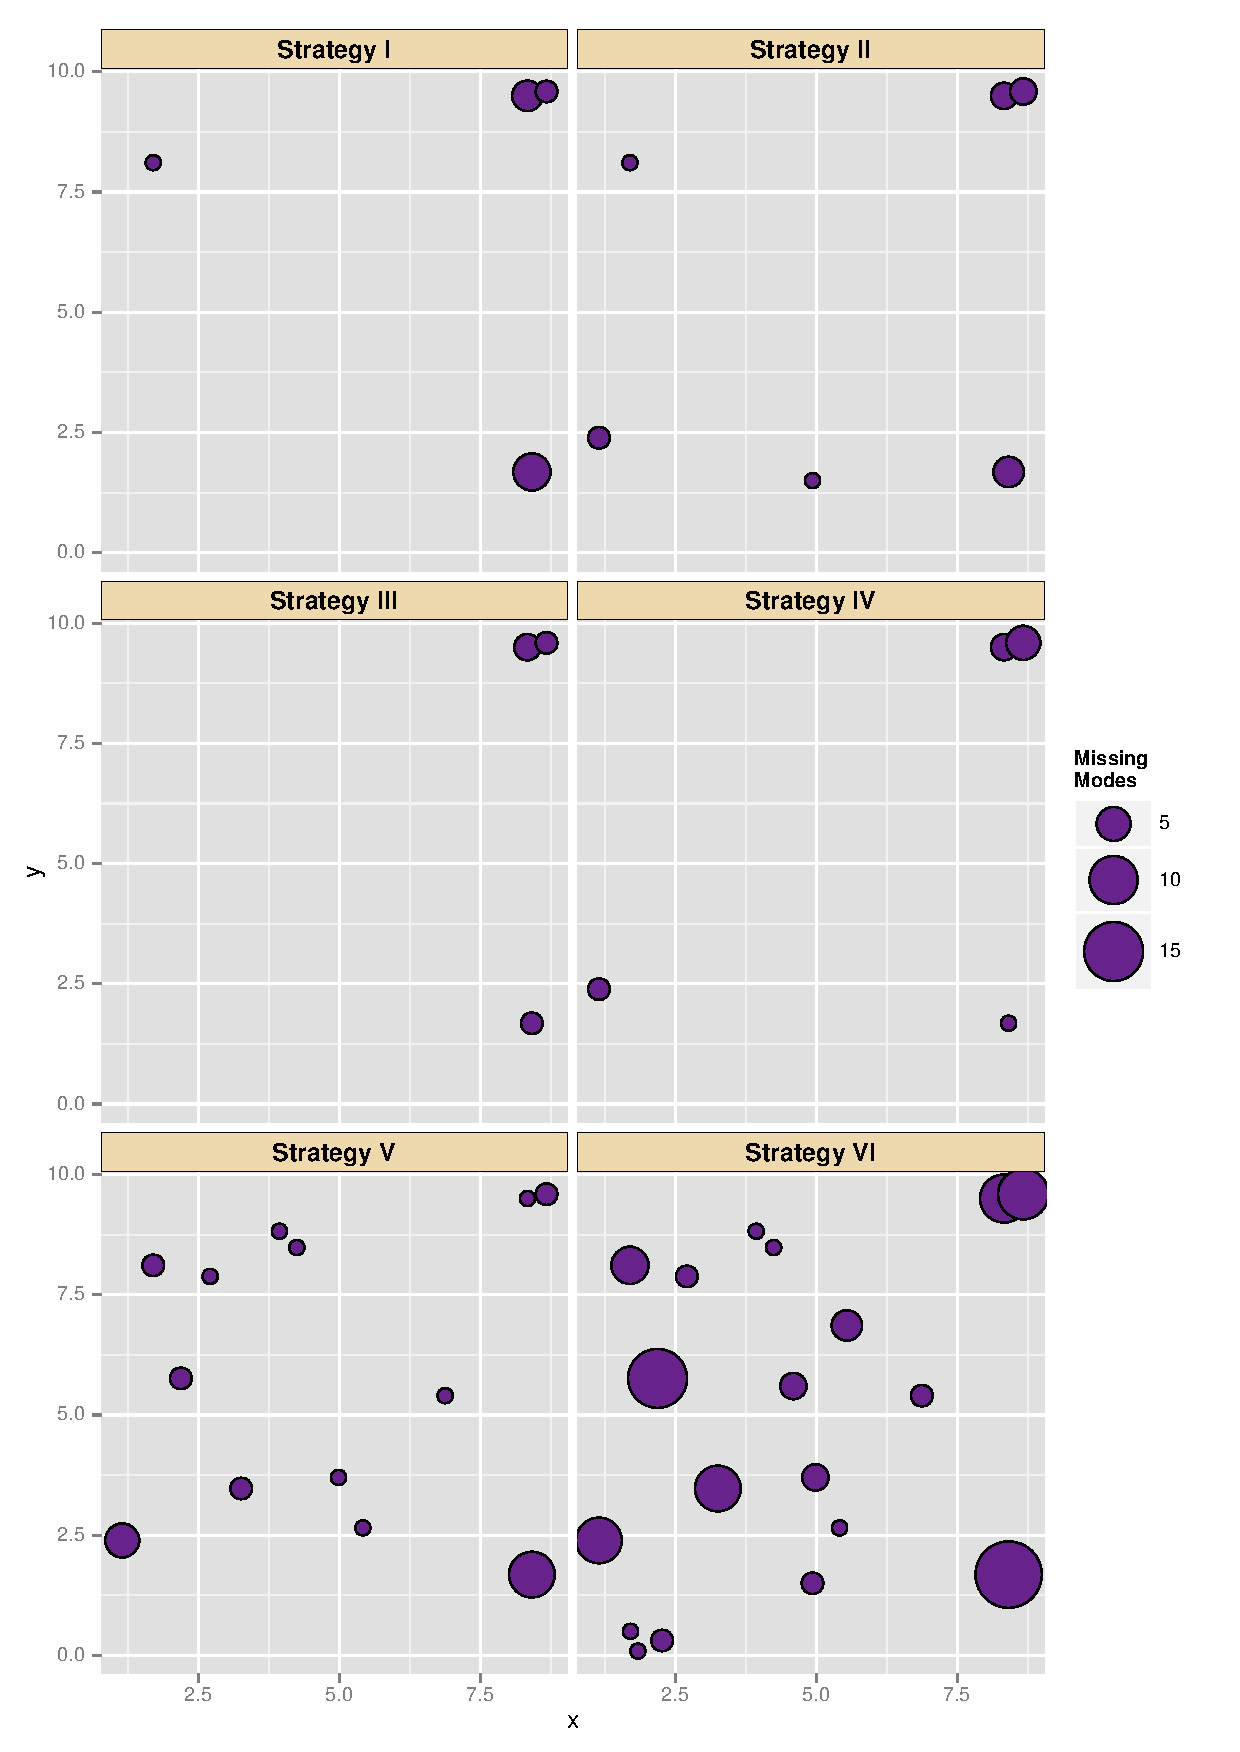
\includegraphics[width=\textwidth,keepaspectratio=TRUE]{./img/ggplotMissingModes.pdf}
	\caption{Missing Modes.}\label{missingModes}
\end{figure}


\begin{figure}[ht]
	\centering 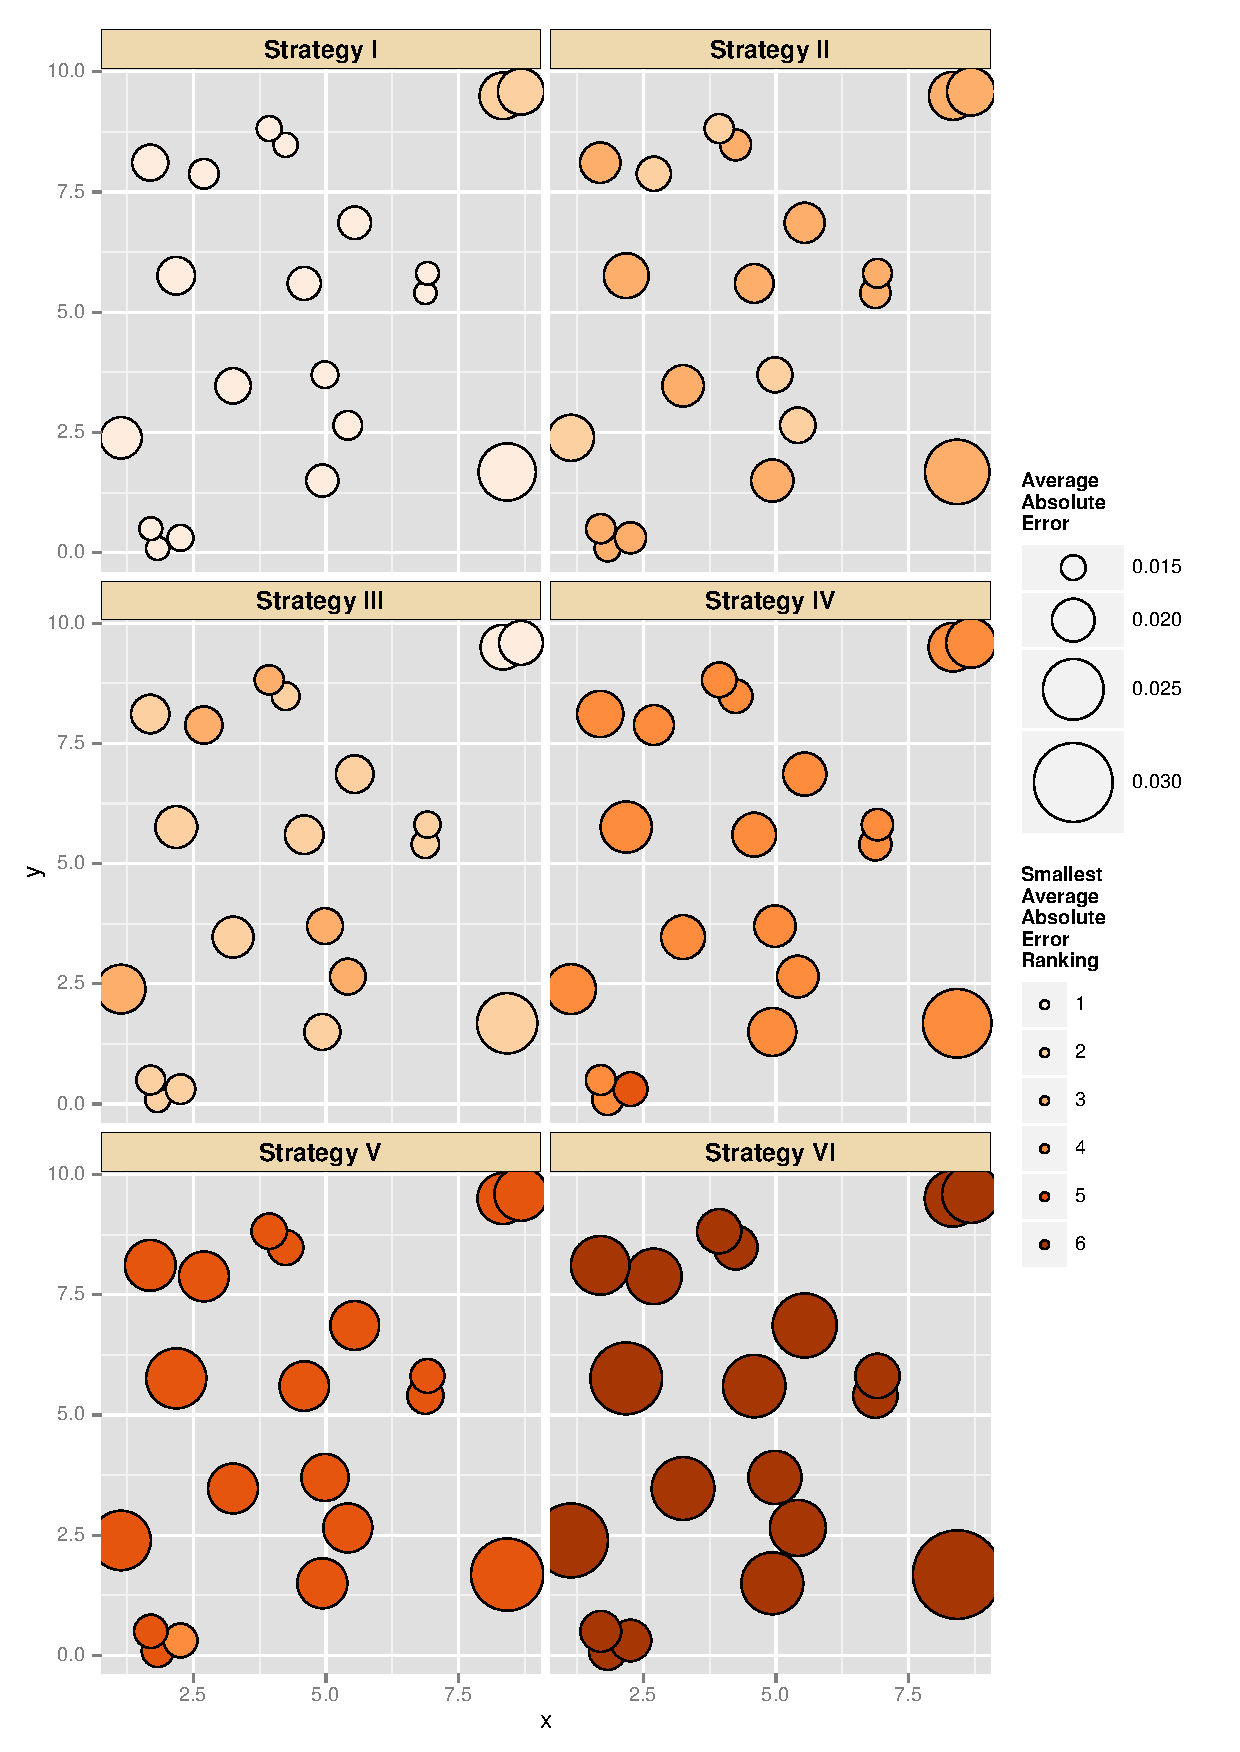
\includegraphics[width=\textwidth,keepaspectratio=TRUE]{./img/ggplotAverageAbsoluteError.pdf}
	\caption{Missing Modes.}\label{missingModes}
\end{figure}

\section{Two modes with different weights}

Another example is inspired by paper by \cite{BaragattiLikelihoodFreeParallelTempering}. The goal is to test different swapping strategies in finding also less accentuated modes of probability. For that reason, the following mixture of normal distributions was considered

\begin{equation*}
f(x) = 
 	\frac{1}{10} \frac{1}{2 \pi \sigma_1^2} \exp \Big( -\frac{ ||x - \mu_1||^2}{2 \sigma_1^2} \Big) +
 	\frac{9}{10} \frac{1}{2 \pi \sigma_2^2} \exp \Big( -\frac{ ||x - \mu_2||^2}{2 \sigma_2^2} \Big)
 	,	
\end{equation*}
where $\sigma_1 = 0.7$ and $\sigma_2 = 0.05$ and the means are 

\begin{table}[ht]
	\centering
	\begin{tabular}{rr}
	  	\hline
			$\mu_1$ & $\mu_2$ \\ 
	  	\hline
			2 & 8 \\ 
			2 & 8 \\ 
	   	\hline
	\end{tabular}
\end{table}



	\bibliographystyle{./bibliography/eccaNoNotes}
	\bibliography{./bibliography/myBooks}


\end{document}

